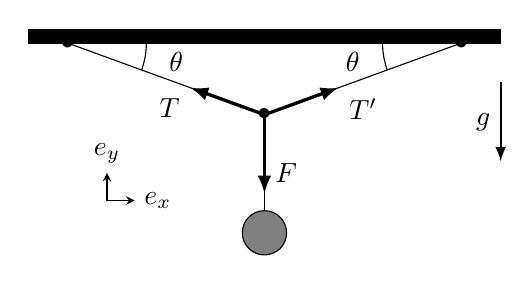
\begin{tikzpicture}[
scale=1,
force/.style={->,>=latex,draw=\JRLblue,very thick,nodes={\JRLblue}},
plane/.style={draw=\JRLblueC,fill=\JRLblueC},
 vecteur/.style={-latex,thick},
]
	\def \thetaUn {20};
	\def \thetaDeux {20};
	\def \AB {5};
	% fil
	\draw ({-tan(\thetaDeux)/(tan(\thetaDeux)+tan(\thetaUn))*\AB},0)node{$\bullet$}--(0,{-tan(\thetaUn)*tan(\thetaDeux)/(tan(\thetaDeux)+tan(\thetaUn))*\AB})--({tan(\thetaUn)/(tan(\thetaDeux)+tan(\thetaUn))*\AB},0)node{$\bullet$};
	% support
	\draw[plane] (-{0.6*\AB},0)rectangle({.6*\AB},5pt); 
	\draw[\JRLblueF] (-{0.6*\AB},0)--({.6*\AB},0);
	
	\draw (0,{-tan(\thetaUn)*tan(\thetaDeux)/(tan(\thetaDeux)+tan(\thetaUn))*\AB})--++(0,-1.5);
	\draw[fill=gray,shift={(0,{-tan(\thetaUn)*tan(\thetaDeux)/(tan(\thetaDeux)+tan(\thetaUn))*\AB})}](0,-1.5) circle(8pt);
	% angles
	\draw[black,shift={({-tan(\thetaDeux)/(tan(\thetaDeux)+tan(\thetaUn))*\AB},0)}] (-\thetaUn:1)arc(-\thetaUn:0:1);
	\draw[black,shift={({tan(\thetaUn)/(tan(\thetaDeux)+tan(\thetaUn))*\AB},0)}] ({180+\thetaDeux}:1)arc({180+\thetaDeux}:180:1);
	\draw[shift={({-tan(\thetaDeux)/(tan(\thetaDeux)+tan(\thetaUn))*\AB},0)}]({-\thetaUn/2}:1.4)node{$\theta$};
	\draw[shift={({tan(\thetaUn)/(tan(\thetaDeux)+tan(\thetaUn))*\AB},0)}]({180+\thetaDeux/2}:1.4)node{$\theta$};
	% forces
	\draw[force] (0,{-tan(\thetaUn)*tan(\thetaDeux)/(tan(\thetaDeux)+tan(\thetaUn))*\AB})--++(0,-1)node[above right]{$\vv{F}$};
	\draw[force] (0,{-tan(\thetaUn)*tan(\thetaDeux)/(tan(\thetaDeux)+tan(\thetaUn))*\AB})--++({180-\thetaUn}:1)node[below left]{$\vv{T}$};
	\draw[force] (0,{-tan(\thetaUn)*tan(\thetaDeux)/(tan(\thetaDeux)+tan(\thetaUn))*\AB})--++(\thetaDeux:1)node[below right]{$\vv{T'}$};
	\draw[vecteur]({0.6*\AB},-.5)--++(0,-1)node[midway,left]{$\vv{g}$} ;
	% point A
	\draw (0,{-tan(\thetaUn)*tan(\thetaDeux)/(tan(\thetaDeux)+tan(\thetaUn))*\AB})node{•}node[above=3pt]{\ptA};
	% base
	\draw[<->,>=stealth,shift={(-2,-2)}](10pt,0)node[right]{$\vv{e_x}$}-|(0,10pt)node[above]{$\vv{e_y}$};
\end{tikzpicture}